\chapter{Análisis del problema}

\section{Solución propuesta}

Como se ha explicado en el Capítulo 1, los peligros del malware en Android son extensos y hay que tener especial cuidado si no queremos que nuestros datos se filtren, sean bloqueados o incluso borrados.

Hemos visto algunos ejemplos de distintas soluciones para detectar malware. Este trabajo se va a centrar en explorar una de ellas, concretamente en una solución que propone un análisis estático que estudia los metadatos de la aplicación contenidos en el \textit{AndroidManifest.xml}: nos vamos a centrar en los permisos peligrosos, aquellos que más arriesgan los datos del usuario. Utilizando la frecuencia con la que las aplicaciones begnigas y el malware utilizan cada uno de estos permisos, se creará un detector en forma de aplicación que clasifique cada aplicación restante instalada en el dispositivo (excepto ella misma) en aplicación benigna o aplicación maliciosa.

En el siguiente capítulo se describirá en detalle la implementación tanto de la aplicación como de los algoritmos utilizados.
 
\section{Análisis de requisitos}

Los requisitos de la aplicación son los siguientes:

\begin{itemize}
	\item \textbf{RF1.} La aplicación debe mostrar el resultado del análisis de las aplicaciones instaladas en el dispositivo.
	\item \textbf{RF2.} Se debe mostrar el nombre de cada app y su correspondiente clasificación.
	\item \textbf{RF3.} El análisis se llevará a cabo solo si el usuario lo solicita.
\end{itemize}

\subsection{Explicación de cada requisito funcional}

\begin{itemize}
	\item \textbf{RF1.} Se mostrará en pantalla un listado de todas las aplicaciones instaladas con su clasificación.
	\item \textbf{RF2.} Para poder identificar cada aplicación se indicará el nombre de ésta además de la etiqueta ``benigna'' o ``maliciosa''.
	\item \textbf{RF3.} El usuario deberá pulsar un botón para activar el análisis. La aplicación nunca funcionará en segundo plano.
\end{itemize}

La estructura a grandes rasgos de la aplicación se puede ver en el siguiente diagrama de clases.

\begin{figure}[H]
\centering
	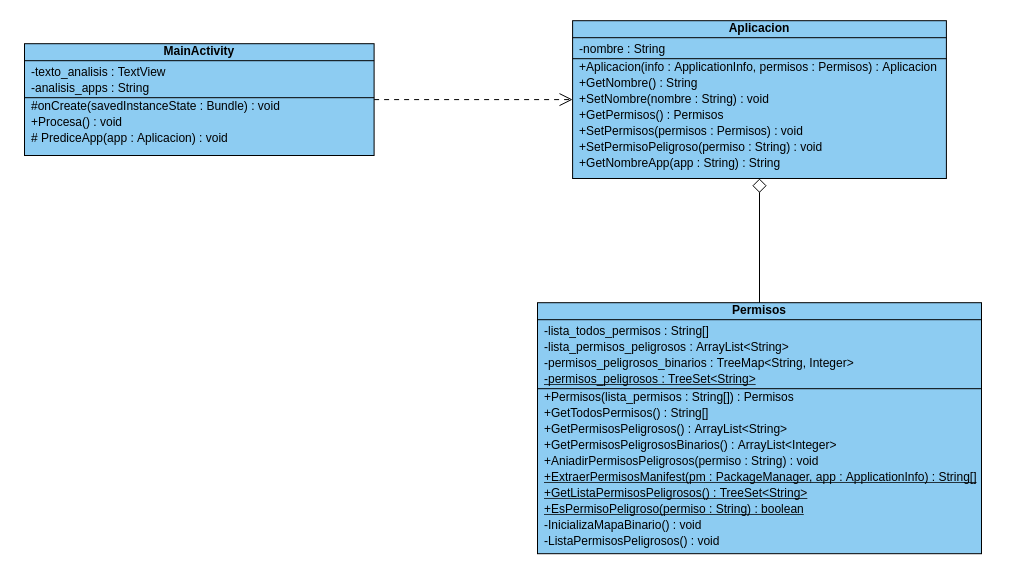
\includegraphics[scale=0.37]{img/uml.png}
	\caption{Diagrama de clases}
\end{figure}

\section{Funcionamiento de los algoritmos de ML}
\label{sec53}

\subsection{Aprendizaje no supervisado: PCA}

El \textit{\href{https://en.wikipedia.org/wiki/Principal_component_analysis}{\textcolor{blue}{Principal Component Analysis}}} o Análisis de Componentes Principales (también llamado PCA), es una técnica que se usa para describir un conjunto de datos en forma de nuevas variables (componentes) que no están relacionadas entre sí. Cada variable da una cantidad de información determinada sobre el problema, por lo que este algoritmo se utiliza para reducir la dimensionalidad del conjunto de datos original; se queda solo con aquellas variables que contienen información suficiente para la resolución del problema.

En este trabajo se ha utilizado la biblioteca \href{https://scikit-learn.org/stable/}{\textcolor{blue}{Scikit Learn}}, que implementa el algoritmo PCA y el SVM. Scikit Learn es una de las bibliotecas de \textit{Machine Learning} más potentes y con mayor variedad de algoritmos disponibles, recomendada para crear modelos ligeros y eficientes que no requieren gran capacidad computacional\hypersetup{citecolor=red}\cite{oreilly}.

Los componentes principales de los datos (representados como un conjunto de puntos en un espacio de coordenadas) son una serie de vectores unitarios donde el vector i-ésimo tiene la dirección de la recta que mejor se ajusta a los datos al mismo tiempo que es ortogonal a los i-1 vectores anteriores. La recta que mejor se ajusta es aquella que minimiza la media de las distancias al cuadrado de los puntos a dicha recta. Esto se traduce en que el PCA cambia ligeramente el conjunto de datos original para quedarse solo con los datos que mejor se ajustan a la recta, lo que significa que en algunas ocasiones se queda solo con unos pocos componentes principales e ignora los demás, manteniendo siempre la mayor variación entre los datos.

En nuestro caso, en este trabajo se ha aplicado el PCA para que el conjunto de permisos original (30 permisos peligrosos) sea reducido de forma que se quede solamente con aquellos permisos que realmente son útiles para diferenciar las aplicaciones entre benignas o maliciosas. Al reducir el número de características, reducimos el ruido que puede confundir al modelo y provocar un sobreajuste a los datos de entrenamiento. Utilizando el PCA nos aseguramos de que el modelo es más genérico.

\subsection{Aprendizaje supervisado: SVM}

Para entrenar el modelo que lleva a cabo la clasificación de las aplicaciones se ha utilizado el algoritmo \textit{\href{https://en.wikipedia.org/wiki/Support-vector_machine}{\textcolor{blue}{Support Vector Machine}}} o Máquina de Vector Soporte, abreviado como SVM. Como se ha explicado ya, este algoritmo es uno de los que mejores resultados arroja en la clasificación de malware. Al igual que para el PCA, se ha utilizado Scikit Learn, por los motivos anteriormente descritos.

El SVM clasifica en dos categorías diferentes un objeto proveniente de un conjunto de datos (de los cuales desconocemos su categoría). Para ello, mediante la búsqueda de un hiperplano separa los datos entre dos subconjuntos con la condición de que debe cumplir con la mayor distancia entre sus fronteras; es decir, se calcula el plano con el cual las distancias de los objetos que hay en el límite de los subconjuntos son máximas. Así, los dos subconjuntos de datos clasificados quedan separados por el hiperplano, uno a cada lado de éste. Se puede ver una representación gráfica en la Figura~\ref{fig:svm}.

\begin{figure}[]
\centering
	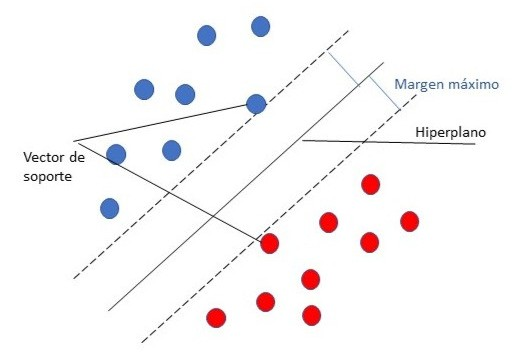
\includegraphics[scale=0.45]{img/svm.jpg}
	\caption{Representación gráfica del funcionamiento del SVM \textit{(Martínez, 2019)}}
	\label{fig:svm}
\end{figure}

Al vector con los los objetos más cercanos al hiperplano se le denomina vector soporte. Las máquinas de vector soporte pueden utilizarse tanto para problemas de regresión como para problemas de clasificación, siendo conceptualmente más apropiados para estos últimos. Están directamente relacionadas con redes neuronales, lo que supone que un modelo bien entrenado suele alcanzar tasas de acierto excelentes. Optimizan la clasificación en dos subconjuntos para crear la mayor diferenciación posible entre categorías. Puesto que este proyecto pretende clasificar una aplicación para hacer que encaje en una de las dos categorías posibles de aplicación (a saber, benigna o maliciosa), este algoritmo es el más adecuado.

Normalmente, no nos encontramos con casos idílicos en los que tenemos dos dimensiones y el hiperplano es recto. Es más, el hiperplano buscado tiene la misma dimensionalidad que el espacio, el cual no tiene por qué ser bidimensional; el número de dimensiones depende del problema concreto (puede llegar a tener infinitas). Además, dependiendo de la distribución de los objetos en el espacio, el hiperplano no tiene por qué ser una línea recta. Puede ser un plano curvo siempre y cuando cumpla con los requisitos de mayor margen entre los objetos frontera y él mismo.

Por tanto, el SVM se enfrenta a varios problemas:

\begin{itemize}
	\item Que haya más de dos variables predictoras en el problema (como es el caso de este trabajo).
	\item Que el hiperplano de separación sea una curva no lineal.
	\item Que los conjuntos no puedan ser totalmente separados ya que, en el caso de serlo, el modelo no puede generalizarse para otros datos (sobreajuste).
	\item Que un objeto pueda ser clasificado en ambas categorías.
\end{itemize}

Por este motivo, el SVM utiliza una \textit{función Kernel} (en este trabajo es una función lineal), que permite convertir un problema de clasificación no lineal en el espacio dimensional original en un problema de clasificación lineal en un espacio dimensional mayor.

